\chapter{Background}
In this chapter, we review the concept of Turing Machines and constructing a parser for a programming language.

\section{Turing Machines}
In this section, we review the definition of Turing Machines and executing a TM on a valid tape.

A \emph{Turing Machine} (TM) is a collection $(Q, \Sigma, \delta, q_0)$, where:
\begin{itemize}
    \item $Q$ is a set of states, including the accept state $q_Y$ and reject state $q_N$;
    \item $\Sigma$ is the set of letters, which does not include the \texttt{blank} symbol;
    \item $\delta \colon Q \setminus \{q_Y, q_N\} \times \Sigma^+ \to Q \times \Sigma^+ \times \{\texttt{left}, \texttt{right}\}$, where $\Sigma^+ = \Sigma \cup \{\texttt{blank}\}$, is the transition function; and
    \item $q_0 \in Q$ is the starting state.
\end{itemize}
We can represent a TM as a directed graph, with vertices as states and edges as transitions. For example, the following is a TM:
\begin{figure}[H]
    \centering
    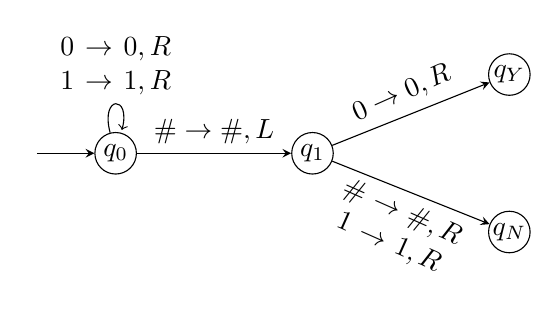
\begin{tikzpicture}
        \node[circle, draw=black, fill=white, inner sep=0pt, minimum size=15pt] (s0) at (0, 0) {$q_0$};
        \node[circle, draw=black, fill=white, inner sep=0pt, minimum size=15pt] (s1) at (2.5, 0) {$q_1$};
        \node[circle, draw=black, fill=white, inner sep=0pt, minimum size=15pt] (sN) at (5, -1) {$q_N$};                
        \node[circle, draw=black, fill=white, inner sep=0pt, minimum size=15pt] (sY) at (5, 1) {$q_Y$};

        \draw[-stealth] (-1, 0) -- (s0);
        \draw[-stealth] (s0) -- node[above] {$\# \to \#, L$} (s1);
        
        \draw[-stealth] (s0) edge[loop above] node[above, text width=2cm, align=center] {$0 \to 0, R$ $1 \to 1, R$} (s0);
        
        \draw[-stealth] (s1) -- node[above, rotate=24] {$0 \to 0, R$} (sY);
        \draw[-stealth] (s1) -- node[below, rotate=-24, text width=2cm, align=center] {$\# \to \#, R$ $1 \to 1, R$} (sN);
    \end{tikzpicture}
    \caption{A Turing Machine that accepts binary numbers divisible by 2.}
\end{figure}
\noindent In this case, the alphabet $\Sigma = \{0, 1\}$. The blank symbol is denoted by $\#$. The initial state is denoted by $q_0$; the accept state $q_Y$ and the reject state $q_N$. Every edge corresponds to an evaluation of the transition function $\delta$, e.g. $\delta(q_0, a) = (q_1, \texttt{blank}, \texttt{right})$.

Let $\Sigma$ be an alphabet. A \emph{tape $T$ on $\Sigma$} is a function $T\colon \mathbb{Z} \to \Sigma^+$. In particular, the tape has infinite entries in both directions. Moreover, $T$ is a \emph{valid tape} if only finitely many symbols on $T$ are not \texttt{blank}, and all the values that can be non-\texttt{blank} are non-\texttt{blank}. That is, there exist integers $a, b$ such that for all $x \in \mathbb{Z}$, $T(x)$ is not \texttt{blank} if and only $x \geq a$ and $x \leq b$. We will represent a tape using a figure. For instance, let $\Sigma = \{0, 1\}$, and let $T$ be the tape on $\Sigma$ given below:
\[T(x) = \begin{cases}
    0 & x \in \{0, 2, 3\} \\
    1 & x \in \{1\} \\
    \texttt{blank} & \text{otherwise}.
\end{cases}\]
Then, the following figure represents the tape $T$:
\begin{figure}[H]
    \centering
    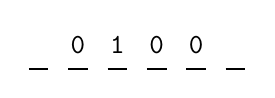
\begin{tikzpicture}
        \draw[thick] (-0.25, 0) -- (0, 0);
        \foreach \x[count=\i] in {0, 1, 0, 0} {
            \draw[thick] (\i*0.5-0.25, 0) -- (\i*0.5, 0);
            \node at (\i*0.5-0.125, 0.3) {\texttt{\x}};
        }
        \draw[thick] (2.25, 0) -- (2.5, 0);
    \end{tikzpicture}
\end{figure}
\noindent We will assume that the first non-blank value is at index 0.

% Note that the following tape would be invalid:
% \begin{figure}[H]
%     \centering
%     \begin{tikzpicture}
%         \draw[thick] (-0.25, 0) -- (0, 0);
%         \foreach \x[count=\i] in {0, 1, 0, , 0} {
%             \draw[thick] (\i*0.5-0.25, 0) -- (\i*0.5, 0);
%             \node at (\i*0.5-0.125, 0.3) {\texttt{\x}};
%         }
%         \draw[thick] (2.75, 0) -- (3, 0);
%     \end{tikzpicture}
% \end{figure}
% \noindent This is because there is a \texttt{blank} symbol between the non-blank symbols.

% TODO: Add reference

A TM can be executed on a tape. Let $M$ be a TM with alphabet $\Sigma$, and let $T$ be a (valid) tape on $\Sigma$. We execute $M$ on $T$ inductively, as follows:
\begin{itemize}
    \item At any point during execution, we maintain 3 objects- a tape on $\Sigma$, a state in $M$ and an index in the tape (called the \emph{tapehead index}). 
    \item At the start, the tape is $T$; the tapehead index is $0$; and the state is the initial state $q_0$. 
    \item At some point during the execution, assume that we have the tape $S$, tapehead index $j$, with \emph{tapehead value} $T(j) = t$, and a non-terminating state $q$ (i.e. not $q_Y$ or $q_N$). Denote $\delta(q, t) = (q', t', \texttt{dir})$. Then, the next state is $q'$, and the next tape $S'$ and the next tapehead index $j'$ are given by:
    \[S'(x) = \begin{cases}
        t' & x = i \\
        S(x) & \text{otherwise},
    \end{cases} \qquad j' = \begin{cases}
        j+1 & \texttt{dir} = \texttt{right} \\
        j-1 & \texttt{dir} = \texttt{left}.
    \end{cases}\]
    If the state $q'$ is not a terminating state, then the execution continues with these 3 objects. Otherwise, execution is terminated with terminating state $q'$.
\end{itemize}

\section{Parser}
TODO
